\section{INTRODUCTION}
Over the last half of the 19th and first decade of the 20th centuries Lane,
Ritter, and Emden codified the earliest mathematical model of stellar
structure, the polytrope (Equation \ref{eqn:polytrope}), in \textit{Gaskugeln}
(Gas Balls) \citep{Emden1907}.

\begin{align}\label{eqn:polytrope}
	\frac{d}{d\xi}\left(\xi^{2}\frac{d\theta}{d\xi}\right) = -\xi^{2}\theta^{n}
\end{align}

Where $\xi$ and $\theta$ are dimensionless parameterizations of radius and
temperature respectively, and $n$ is known as the polytropic index. Despite this
early work, it wasn't until the late 1930s and early 1940s that the full set of
equations needed to describe the structure of a steady state,
radially-symmetric, star (known as the equations of stellar structure) began to
take shape as proton-proton chains and the Carbon-Nitrogen-Oxygen cycle were,
for the first time, seriously considered as energy generation mechanisms
\citep{Cowling1966}. Since then, and especially with the proliferation of
computers in astronomy, the equations of stellar structure have proven
themselves an incredibly predictive set of models.  

There are currently many stellar structure codes \citep[e.g.][]{Dotter2008,
Kovetz2009, Paxton2011} which integrate the equations of stellar structure ---
in addition to equations of state and lattices of nuclear reaction rates ---
over time to track the evolution of an individual star. The Dartmouth Stellar
Evolution Program (DSEP) \citep{Chaboyer2001, Bjork2006, Dotter2008} is one
such, well tested, stellar evolution program.

Here we propose to model low-mass stars in both the local solar neighborhood
and in globular clusters using DSEP. This work will primarily extend our
understanding of stellar physics in two areas: the effects of chemically
self-consistency on stellar models and time evolution of the core-convective
instabilities which ultimatly are belived to result in the observed paucity of
stars at a Gaia G magnitude of $\sim$10. [NEED CITATIONS IN THIS PARAGRAPH]

Low mass stars form an important component of the stellar population, with
stars less than [MASS HERE] making up more than 70\% of stars in the galaxy
[CITE]. Moreover, due to their long lives, low-mass stars provide essential
constraints on ages of various stellar populations [CITE]. In globular
clusters, where all stars are coeval to one of a limited number of populations,
low mass stars provide the vast majority of constraints when fitting ischrones [CITE].
Additionally, stars around the fully-convective transition mass show
age-dependent core-convective instabilities [CITE].

\subsection{Globular Clusters}

Globular clusters in the local universe are primarly composed of old and
consequently low-mass stars. For decades, prevaling thought had it globular
clusters were composed of a single stellar population born from a preisten
interstellar medium. This was supported by visibly tight main sequences and
clear main sequence turn offs in optical CMDs \citep[Figure
\ref{fig:M3CMD}][]{Sandage1953}. These early studies either did not handel or
had very large photometric uncertanties and therefore they were unable to
discriminate beteween CMD features with small separations,

\begin{figure}
	\centering
	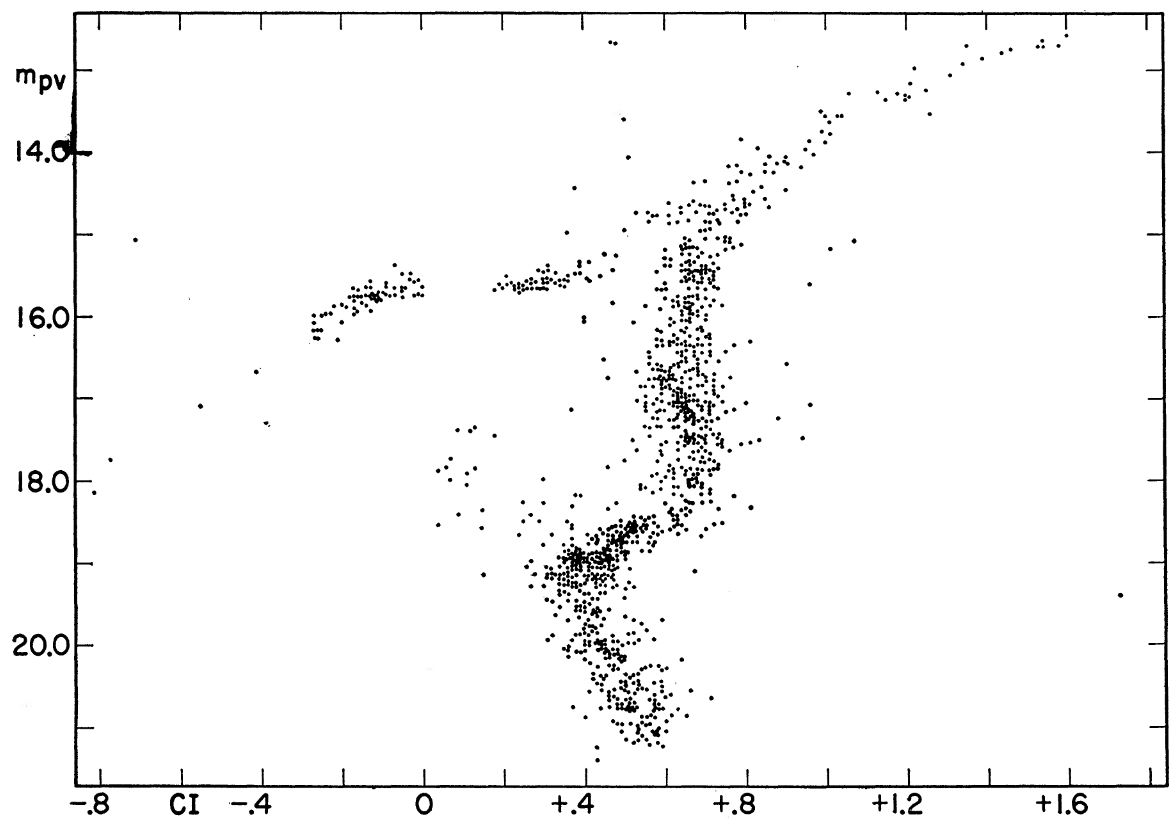
\includegraphics[width=0.75\textwidth]{src/Figures/Gould53.png}
	\caption{$m_{pg}$ - $m_{pv}$ color-magnitude diagram for the globular cluster M3.}
	\label{fig:M3CMD}
\end{figure}

[SOMETHING ABOUT EARLY SPECTROSCOPIC INDICATIONS OF MPs]

With the presicion photometric measurements, degenerecies between noise and
intrinsic scatter were broken and it became clear that globular clusters are
almost universally composed of multiple stellar populations (MPs). [GRAB SOME
TEXT FROM THE NGC 2808 SECTION FOR HERE].

\subsection{Local Solar Neighborhood}
\citet{Jao2018} discovered a novel feature in the Gaia Gp-Rp color-magnitude
diagram. Around $M_{G}=10$ there is an approximatly 17\% decreas in stellar
density of the volume complete sample of stars \citeauthor{Jao2018} considered.
Subsequently, this has become known as either the Jao Gap, or Gaia M dwarf Gap.
Section \ref{} will go into more detail regarding the physics belived to
underpin this feature; however, in brief convective instabilities in the core
are belived to form for stars straddeling the fully convective transition mass.
These instabilities result in stars preferentially falling to either side of
the gap location.

Stellar modeling has been sucsessful in reproducing the Jap Gap and, with these
models, we have begun to constrain parameters which constrain gap location. For
example, it is now well documented that a stars metallicity can affect the gap
color by up to [HOW MUCH DID GREG FIND/CHECK FOR OTHER PAPERS ON THIS]. 

Initial testting which we have done using DSEP along with work by [PAPER] also
indicated the Jao Gap's color sensitivity to age. We observe that as models age
the Jao Gap moves [DIRECTION OF MOVMENT IN MAG AND COLOR SPACE].

The OPAL opacity tables in particular are very widely used by current
generation stellar evolution programs (in addition to current generation
stellar model and isochrone grids). However, they are no longer the most up
date elemental opacities. Moreover, the generation mechanism for these tables,
a webform, is no longer reliably online.  Consequently, it makes sense to
transition to more modern opacity tables with a more stable generation
mechanism.

Here we will present work transitioning DSEP from OPAL opacities to opacities
based on measurements from Los Alamos national Labs T-1 group
\citep[OPLIB][]{Colgan2016}. Moreover, we will present two projects which are
in large part reliant on these updated opacities. For the first project we
investigate the affects of chemically self consistent modeling of multiple
populations within the globular cluster NGC 2808, and for the second project we
present the effects of the OPLIB opacities on the location of the recently
discovered Gaia M-dwarf gap.

This paper is organized as follows. In Section \ref{sec:opac} we outline some
basic information about OPLIB opacities, how we query them, and how we modify
them to work with DSEP. In Section \ref{sec:2808} we discuss scientific
background of the first project along with the current work done towards its
goal. Finally, in Section \ref{sec:Jao} we present our findings on the effects
of OPLIB opacities on the location of the Gaia M-dwarf gap.





